\documentclass[a4paper,12pt]{article}

    % Layout
    \usepackage[
        a4paper,
        left=15mm,
        right=15mm,
        top=15mm,
        bottom=15mm]{geometry}
    \usepackage{multicol}
    \setlength\columnsep{20pt}
    %\usepackage{fancyhdr}

    % Català
    \usepackage[catalan]{babel}
    \usepackage[utf8]{inputenc}
    \usepackage[T1]{fontenc}

    % Setting up a sans-serif typeface for the whole document
    \usepackage{microtype}
    \usepackage{paratype}
    \renewcommand{\familydefault}{\sfdefault}

    \usepackage{bbding}

    %Definició de la ela geminada per tal que accepti el punt volat del teclat
    \def\xgem{%
        \ifmmode
            \csname normal@char\string"\endcsname l%
        \else
            \leftllkern=0pt\rightllkern=0pt\raiselldim=0pt
            \setbox0\hbox{l}\setbox1\hbox{l\/}\setbox2\hbox{.}%
            \advance\raiselldim by \the\fontdimen5\the\font
            \advance\raiselldim by -\ht2
            \leftllkern=-.25\wd0%
            \advance\leftllkern by \wd1
            \advance\leftllkern by -\wd0
            \rightllkern=-.25\wd0%
            \advance\rightllkern by -\wd1
            \advance\rightllkern by \wd0
            \allowhyphens\discretionary{-}{}%
            {\kern\leftllkern\raise\raiselldim\hbox{.}%
            \kern\rightllkern}\allowhyphens
        \fi
    }
    \def\Xgem{%
        \ifmmode
            \csname normal@char\string"\endcsname L%
        \else
            \leftllkern=0pt\rightllkern=0pt\raiselldim=0pt
            \setbox0\hbox{L}\setbox1\hbox{L\/}\setbox2\hbox{.}%
            \advance\raiselldim by .5\ht0
            \advance\raiselldim by -.5\ht2
            \leftllkern=-.125\wd0%
            \advance\leftllkern by \wd1
            \advance\leftllkern by -\wd0
            \rightllkern=-\wd0%
            \divide\rightllkern by 6
            \advance\rightllkern by -\wd1
            \advance\rightllkern by \wd0
            \allowhyphens\discretionary{-}{}%
            {\kern\leftllkern\raise\raiselldim\hbox{.}%
            \kern\rightllkern}\allowhyphens
        \fi
    }
    \DeclareTextCommand{\textperiodcentered}{T1}[1]{%
        \ifnum\spacefactor=998
            \Xgem
        \else
            \xgem
        \fi#1}

    % Imatges
    \usepackage{graphicx}
    \usepackage{subfigure}

    % Mates
    \usepackage{amsthm, amsmath, amssymb, amsfonts}

    % Sagnats
    \usepackage{parskip}
    \frenchspacing

    % Taules
    \usepackage{array}
    \newcommand{\PreserveBackslash}[1]{\let\temp=\\#1\let\\=\temp}
    \newcolumntype{C}[1]{>{\PreserveBackslash\centering}p{#1}}
    \newcolumntype{R}[1]{>{\PreserveBackslash\raggedleft}p{#1}}
    \newcolumntype{L}[1]{>{\PreserveBackslash\raggedright}p{#1}}

    % Links
    \usepackage[pagebackref=false, hidelinks]{hyperref}
    \hypersetup {
        pdfauthor    = {Carlos Luna-Mota},
        pdfsubject   = {The Egyptian Tangram - Printable Edition}
        pdftitle     = {The Egyptian Tangram - Printable Edition},
        pdfkeywords  = {Tangram, Tangram Egipci, Egyptian Tangram, Tangram Egipcio, Ägyptischer Tangram, Tangram Égyptien},
        pdfcreator   = {LaTeX},
        pdfproducer  = {pdflatex, bibtex, ghostscript \& python}
    }

\begin{document}
    \thispagestyle{empty}
    \begin{center}
        \raisebox{14ex}{\rotatebox{90}{\fontsize{40}{50}\ScissorRightBrokenBottom}}\hspace{-1.2ex}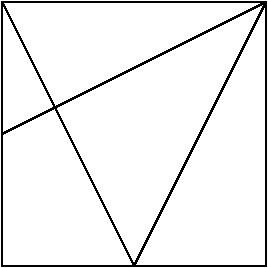
\includegraphics[height=12.5cm]{figures/figura017.pdf}
        \hspace{1.5ex}\raisebox{10ex}{\rotatebox{90}{\normalsize \textbf{\href{https://github.com/CarlosLunaMota/The-Egyptian-Tangram}{Egyptian Tangram}} --- \href{https://creativecommons.org/licenses/by-nc-sa/4.0/}{
\includegraphics[scale=0.15]{cc/cc.pdf}
\includegraphics[scale=0.15]{cc/by.pdf}
\includegraphics[scale=0.15]{cc/nc.pdf}
\includegraphics[scale=0.15]{cc/sa.pdf}}
    \href{mailto:carlos.luna@mmaca.cat}{Carlos Luna-Mota}}}\hspace{2ex}\phantom{m} 
    \end{center}

    \vspace{1.5em}

    \begin{center}
        \begin{tabular}{lccc}
                \raisebox{0.0ex}{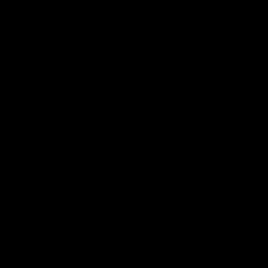
\includegraphics[scale=0.4]{figures/figura022a.pdf}} \;\;&
            \;\;\raisebox{0.0ex}{
\includegraphics[scale=0.4]{figures/figura022j.pdf}} \;\;&
            \;\;\raisebox{0.0ex}{
\includegraphics[scale=0.4]{figures/figura022l.pdf}} \;\;&
            \;\;\raisebox{0.0ex}{
\includegraphics[scale=0.4]{figures/figura022u.pdf}} \\[1.0ex] 
                \raisebox{2.0ex}{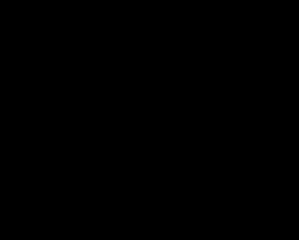
\includegraphics[scale=0.4]{figures/figura022b.pdf}} \;\;&
            \;\;\raisebox{1.6ex}{
\includegraphics[scale=0.4]{figures/figura022m.pdf}} \;\;&
            \;\;\raisebox{0.0ex}{
\includegraphics[scale=0.4]{figures/figura022p.pdf}} \;\;&
            \;\;\raisebox{1.6ex}{
\includegraphics[scale=0.4]{figures/figura022i.pdf}} \\[0.250ex]
                \raisebox{0.0ex}{
\includegraphics[scale=0.4]{figures/figura022c.pdf}} \;\;&
            \;\;\raisebox{0.0ex}{
\includegraphics[scale=0.4]{figures/figura022n.pdf}} \;\;&
            \;\;\raisebox{0.0ex}{
\includegraphics[scale=0.4]{figures/figura022t.pdf}} \;\;&
            \;\;\raisebox{0.0ex}{
\includegraphics[scale=0.4]{figures/figura022h.pdf}} \\[1.5ex]
                \raisebox{0.0ex}{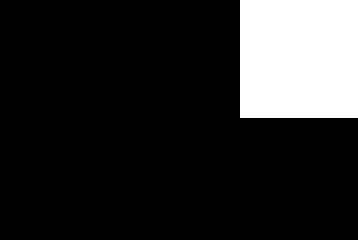
\includegraphics[scale=0.4]{figures/figura022e.pdf}} \;\;&
            \;\;\raisebox{0.0ex}{
\includegraphics[scale=0.4]{figures/figura022o.pdf}} \;\;&
            \;\;\raisebox{0.0ex}{
\includegraphics[scale=0.4]{figures/figura022q.pdf}} \;\;&
            \;\;\raisebox{0.0ex}{
\includegraphics[scale=0.4]{figures/figura022g.pdf}} \\
        \end{tabular}
    \end{center}

    \vspace{2em}
    
    \qquad\;\raisebox{1ex}{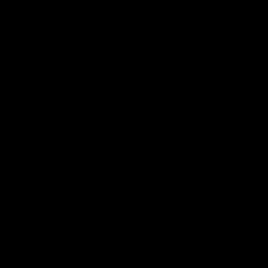
\includegraphics[height=8ex]{figures/figura022a.pdf}\quad\raisebox{3ex}{
\includegraphics[scale=0.1]{figures/figura022t.pdf}}\quad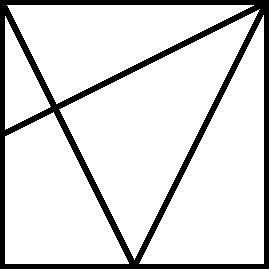
\includegraphics[height=8ex]{figures/figura021a.pdf}\quad
\includegraphics[height=8ex]{figures/figura021b.pdf}\quad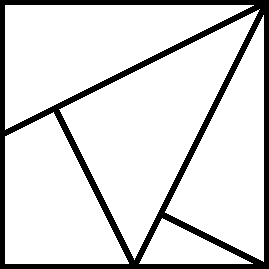
\includegraphics[height=8ex]{figures/figura021c.pdf}}
    \hspace{10ex}\href{https://mmaca.cat/}{
\includegraphics[scale=0.75]{figures/mmaca.png}}
\end{document}
